\documentclass[../TakeYourPill.tex]{subfiles}
\graphicspath{{\subfix{images/}}}

\begin{document}

Všechny data jsem se rozhodl ukládat do lokální databáze\footnote{Nacházející se na zařízení uživatele.}, ze které je mohu efektivně získávat. Pro práci z databází používám jazyk \textit{SQL} v implementaci \textit{SQLite} pod abstraktní vrstvou knihovny \textit{Room} \cite{room}. Tato knihovna mi umožnila jednoduchou práci s databází a jejími tabulkami, aniž bych se musel zabývat vytvářením tabulek, konverzí základních typů nebo manuálními aktualizacemi zobrazených dat. 

Jelikož knihovna plně podporuje funkce jazyka Kotlin zvané \textit{Flow} a \textit{coroutine}, nemusel jsem složitě vymýšlet a programovat asynchronním fungováním databáze. Pokud mám návratovou hodnotu metody v databázové vrstvě nastavenou na \texttt{Flow<T>}, kde \texttt{T} je jakýkoliv datový typ, získávám z ní aktualizace po celou dobu \enquote{sbírání}\footnote{Z anglického výrazu \textit{collect}.} hodnoty této metody. \textit{Coroutiny} nám narozdíl od \textit{Flow} neumožňují sbírat data kontinuálně, můžeme s nimi avšak v jakémkoliv \enquote{coroutinním contextu}\footnote{Z anglického výrazu \textit{Coroutine Context}.} pracovat, jako bychom pracovali s metodami synchronními. Pro nastavení této vlastnosti na metodě se před její definici napíše klíčové slovo \texttt{suspend}. Všechny tyto možnosti nám umožní práci s daty přesunout z hlavního vlákna na vlákna jiná\footnote{V některých případech nemusí jít ani o vlákno, o toto se stará Kotlin jako takový.}. Přesunutí je důležité, aby aplikace běžela svižně, neměla záseky a Android nezobrazoval uživateli varování, že aplikace nereaguje.

Abych mohl začít \textit{Room} používat, nejprve jsem musel vytvořit abstraktní třídu mojí databáze. Databáze obsahuje entity (tabulky), které jsou definovány datovými třídami \texttt{PillEntity}, \texttt{Reminder} a \texttt{History}. Ke každé tabulce jsem vytvořil rozhraní označované jako \enquote{DAO} neboli \enquote{Database Access Object}, umožňující přímý přístup do databáze. V tomto rozhraní definujeme jaké metody můžeme volat na tabulce (popř. databázi) a jejich SQL příkazy. Příklad takového rozhraní by byl následující (vyjmuto z \texttt{PillDao}):

\setmonofont{JetBrains Mono}
\begin{lstlisting}[language=Kotlin]
@Dao
interface PillDao {
    @Transaction
    @Query("SELECT * FROM pill WHERE deleted = 0 ORDER BY pillId ASC")
    fun getEverythingFlow(): Flow<List<Pill>>
    ...
}
\end{lstlisting}
\setmonofont{Latin Modern Mono}

Na tomto příkladu můžeme vidět, že \textit{Room} podporuje i automatické transakce. \texttt{Pill} totiž není databázová entita, ale relační třída, která spojuje entity \texttt{Reminders} a \texttt{PillEntity}. Získáme tak snadno přistup ke všem připomínkám u daného léku bez nutnosti psát \texttt{INNER JOIN} ručně. Aby třída \texttt{Pill} propojení umožňovala, musíme jí zapsat takto:

\setmonofont{JetBrains Mono}
\begin{lstlisting}[language=Kotlin]
data class Pill(
    @Embedded val pillEntity: PillEntity,
    @Relation(
        parentColumn = "pillId",
        entityColumn = "pillId"
    )
    var reminders: List<Reminder>
)
\end{lstlisting}
\setmonofont{Latin Modern Mono}

Pokud bychom chtěli do databáze ukládat hodnoty, s kterými si \textit{Room} nebo \textit{SQL} neporadí, musíme je nejdříve převést na hodnoty, kterým tyto knihovny budou rozumět. V mém případě se jednalo o uložení fotografie, barvy léku a času u připomínky. Pro vytvoření takovýchto konvertorů si definujeme speciální třídu, jejíž metody budou anotované pomocí \texttt{@TypeConverter}. Tuto třídu přiřadíme k databázi, když databázi definujeme. Pro každou vlastní hodnotu uloženou do databáze musíme mít dvě metody; jednu na převod do formátu, kterému rozumí databáze a druhou na převod zpátky do původního formátu. Například pro uložení třídy \texttt{Calendar}, kterou aplikace hojně využívá pro práci s časem, jsem napsal následující konvertory:

\begin{minipage}{\linewidth}
\setmonofont{JetBrains Mono}
\begin{lstlisting}[language=Kotlin]
@TypeConverter
fun toCalendar(millis: Long?) = millis?.let {
    Calendar.getInstance().apply { timeInMillis = it }
}

@TypeConverter
fun fromCalendar(calendar: Calendar?) = calendar?.timeInMillis
\end{lstlisting}
\setmonofont{Latin Modern Mono}
\end{minipage}

Tímto definujeme jaký formát se uloží do tabulky, v tomto případě se ze třídy \texttt{Calendar} stane \texttt{Long}, jehož hodnota bude čas vyjádřený v počtu milisekund (pravděpodobně od 1.1.1970, záleží na typu kalednáře/lokalizaci zařízení). 

Pro grafické znázornění jsem vytvořil následující digram databáze:

\begin{figure}[h]
\centering
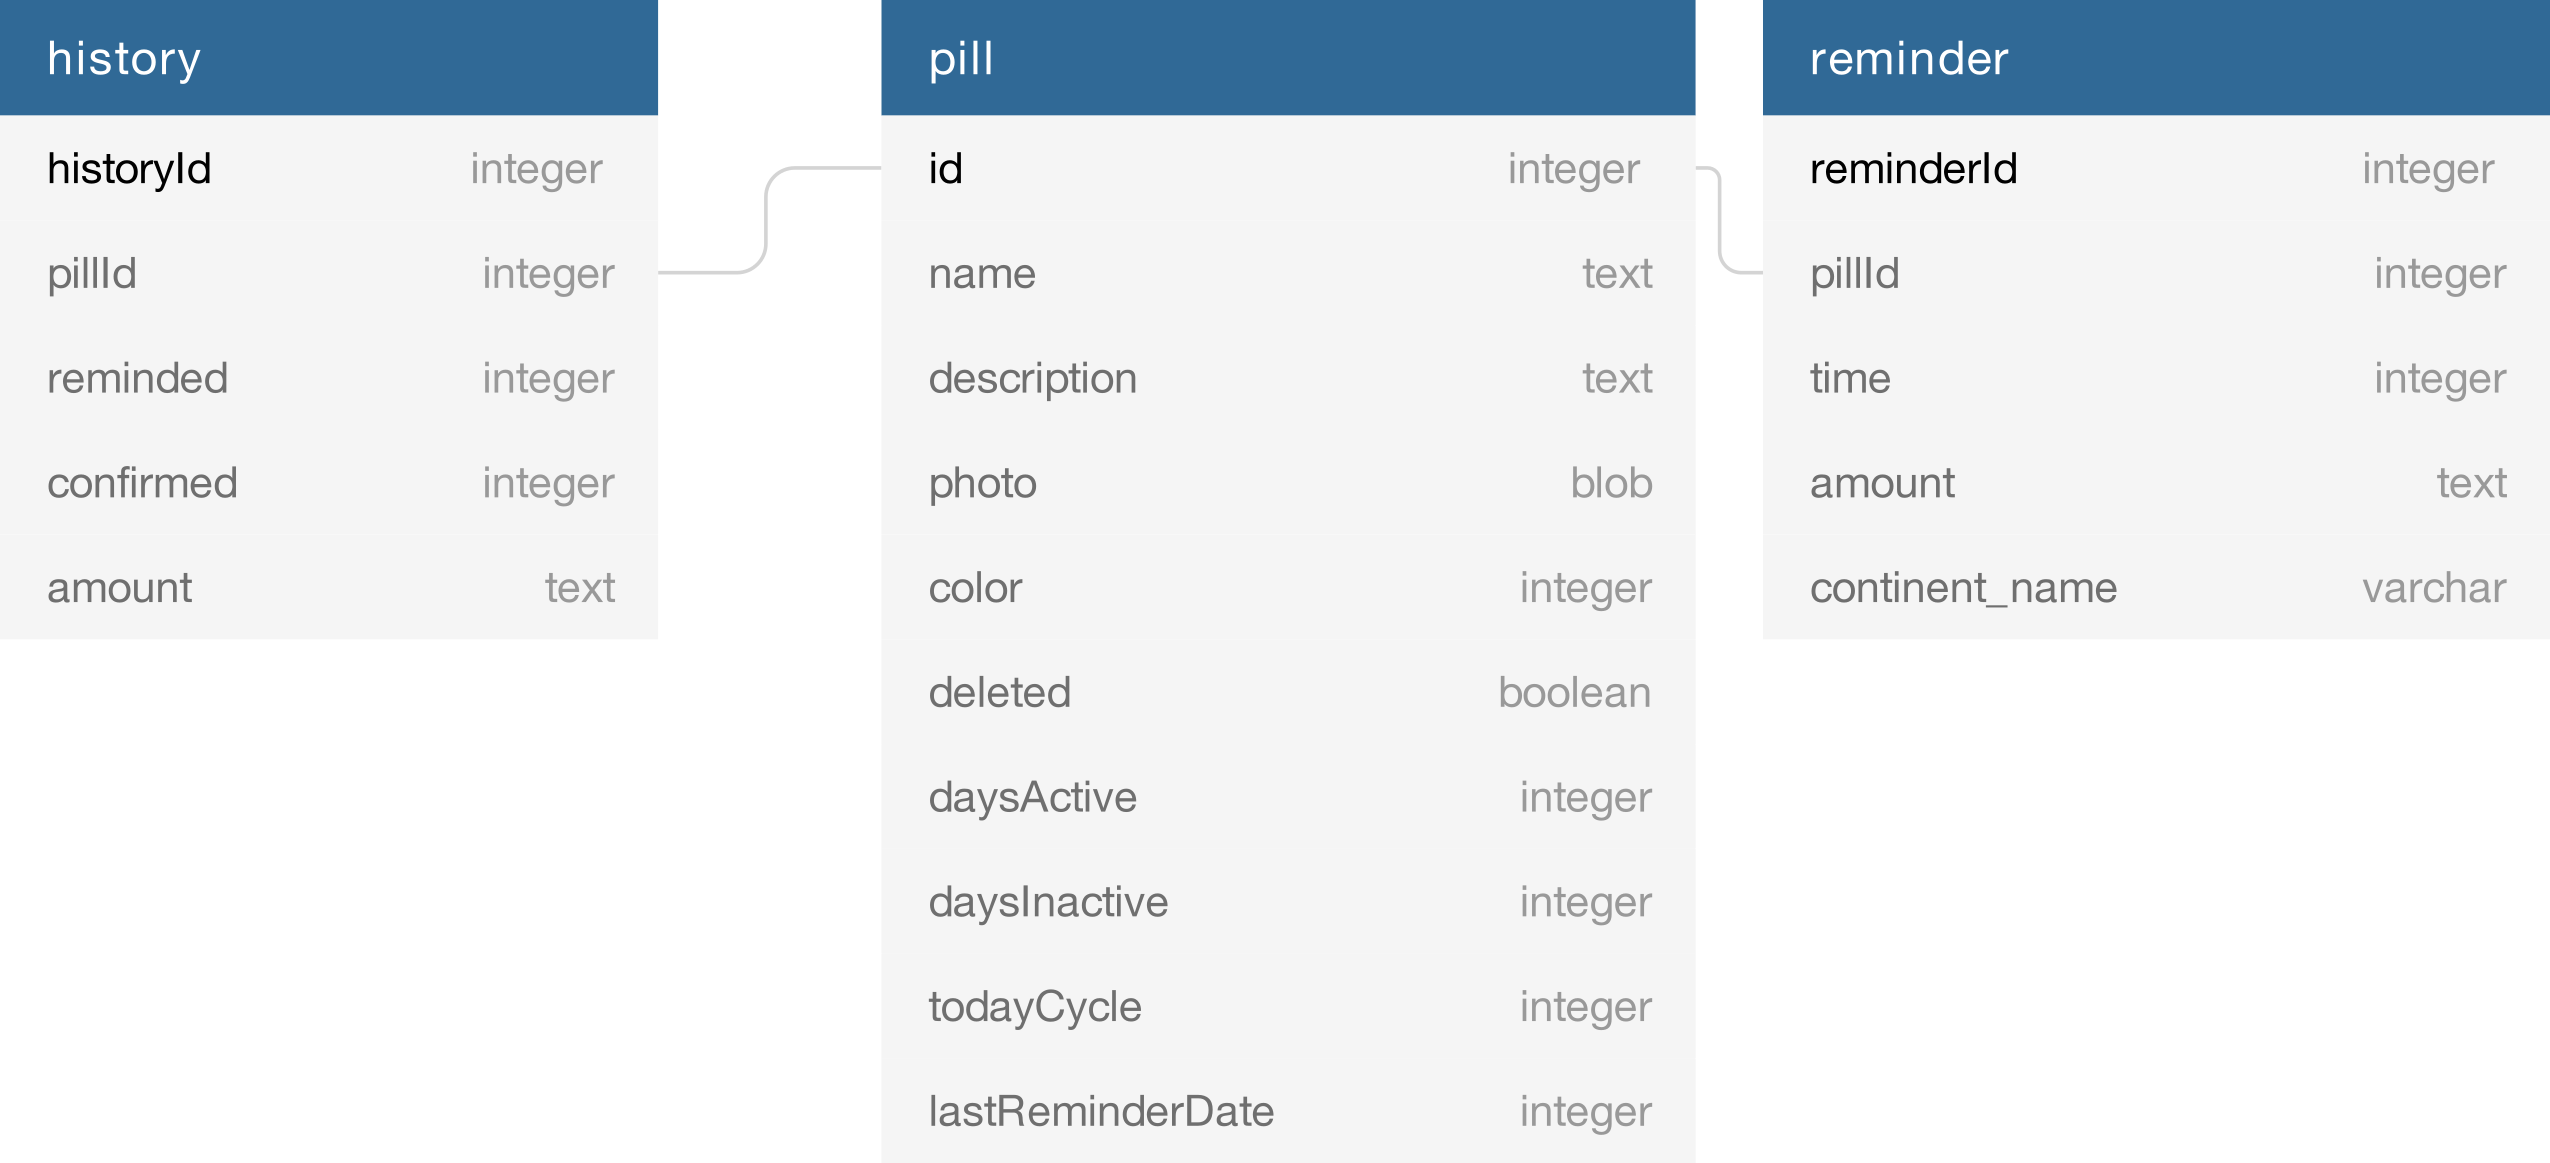
\includegraphics[width=\textwidth]{database.png}
\caption{Databázový diagram vytvořený pomocí stránky \url{https://dbdiagram.io/}}
\end{figure}

\end{document}
